%%%%%%%%%%%%%%%%%%%%%%%%%%%%%%%%%%%%%%%%%%
% Master Thesis 
% Polina Polunina
% October 2022 
%
% License:
% CC-BY-SA 4.0 -- Creative Commons Attribution-ShareAlike 4.0 International
% https://creativecommons.org/licenses/by-sa/4.0/legalcode
%%%%%%%%%%%%%%%%%%%%%%%%%%%%%%%%%%%%%%%%%%
\section{Appendix} \label{sec:appendix}
    \subsection{Galaxy histories} \label{sec:appendix:galaxy-hist}
    \subsubsection{Galaxy history links for Freyja-based branch on real datasets}
    California, US (PRJNA661613): \\
   \url{https://usegalaxy.eu/u/polina/h/sf-dataset-prjna661613-covid-19-variation-analysis-on-wgs-pe-data}\\
    Wales and Northwest England, UK (PRJEB42191): \\
    \url{https://usegalaxy.eu/u/polina/h/uk-dataset-COJAC-prjeb42191-covid-19-variation-analysis-on-artic-pe-data-1}\\
    Ontario, Canada (PRJNA824537): \\
    \url{https://usegalaxy.eu/u/polina/h/ca-dataset-freyja-prjna824537-covid-19-variation-analysis-on-artic-pe-data}\\
    Washington, US (PRJNA765346): \\
    \url{https://usegalaxy.eu/u/polina/h/us-dataset-freyja-prjna765346-covid-19-variation-analysis-on-artic-pe-data-1-1-1-1}

    \subsubsection{Galaxy history links for COJAC-based branch on real datasets}
    Wales and Northwest England, UK (PRJEB42191): \\
    \url{https://usegalaxy.eu/u/polina/h/uk-dataset-COJAC-prjeb42191-covid-19-variation-analysis-on-artic-pe-data-1}\\
    Ontario, Canada (PRJNA824537): \\
    \url{https://usegalaxy.eu/u/polina/h/ca-dataset-COJAC-prjna824537-covid-19-variation-analysis-on-artic-pe-data}\\
    Washington, US (PRJNA765346): \\
    \url{https://usegalaxy.eu/u/polina/h/us-dataset-COJAC-prjna765346-covid-19-variation-analysis-on-artic-pe-data}
    
    \subsection{Listings}
\begin{lstlisting}[language=python, caption=python script to compute the overall lineage abundances proportions of considered lineages in mock dataset for Freyja output, label=list:methods:freyja-vocs-abundances]
#create a dataframe of lineage abundances for freyja
df_fr = (pd.read_csv("data/galaxy-data/freyja_aggregated_data.tsv", sep='\t')
             # remove columns
             .drop((['summarized','resid', 'coverage']), axis=1))
            
df_fr.insert(3,'fr_delta', 0.0)
df_fr.insert(4,'fr_ba1', 0.0)
df_fr.insert(5,'fr_ba2', 0.0)
df_fr.insert(6,'fr_other', 0.0)

#compute the overall lineage abundances proportions for delta, BA1, BA2, and other for Freyja output
delta = ['B.1.617.2', 'AY']
fr_dic = {}

for ind in df_fr.index:
    ab_d = 0.0
    ab_ba1 = 0.0
    ab_ba2 = 0.0
    ab_o = 0.0
    l = df_fr['lineages'][ind]
    a = df_fr['abundances'][ind]
    dic = dict(zip(l.split(), [float(i) for i in a.split()]))
    for i, j in dic.items():
        if any(x in i for x in delta):
            ab_d += j
            x = {'delta': ab_d}
            fr_dic.update(x)
            df_fr['fr_delta'][ind] = ab_d
        elif 'BA.1' in i:
            ab_ba1 += j
            x = {'ba1': ab_ba1}
            fr_dic.update(x)
            df_fr['fr_ba1'][ind] = ab_ba1
        elif 'BA.2' in i:
            ab_ba2 += j
            x = {'ba2': ab_ba2}
            fr_dic.update(x)
            df_fr['fr_ba2'][ind] = ab_ba2
        else:
            ab_o += j
            x = {'other': ab_o}
            fr_dic.update(x)
            df_fr['fr_other'][ind] = ab_o
        
df_fr = df_fr.drop((['lineages','abundances']), axis=1)
\end{lstlisting}
    \subsection{Further figures}
        \subsubsection{Existing Galaxy workflows that were not changed} \label{sec:appendix:figures:wfs}
        Other existing Galaxy workflows for SARS-CoV-2 clinical data surveillanve that were not taken as a basis for improvement and repurposing in this thesis are presented in \cref{fig:further:ont-wf} and \cref{fig:further:illumina-wf}.
        \begin{landscape}
        \centering\vspace*{\fill}
        \begin{figure}[ht!]
        	\centering
            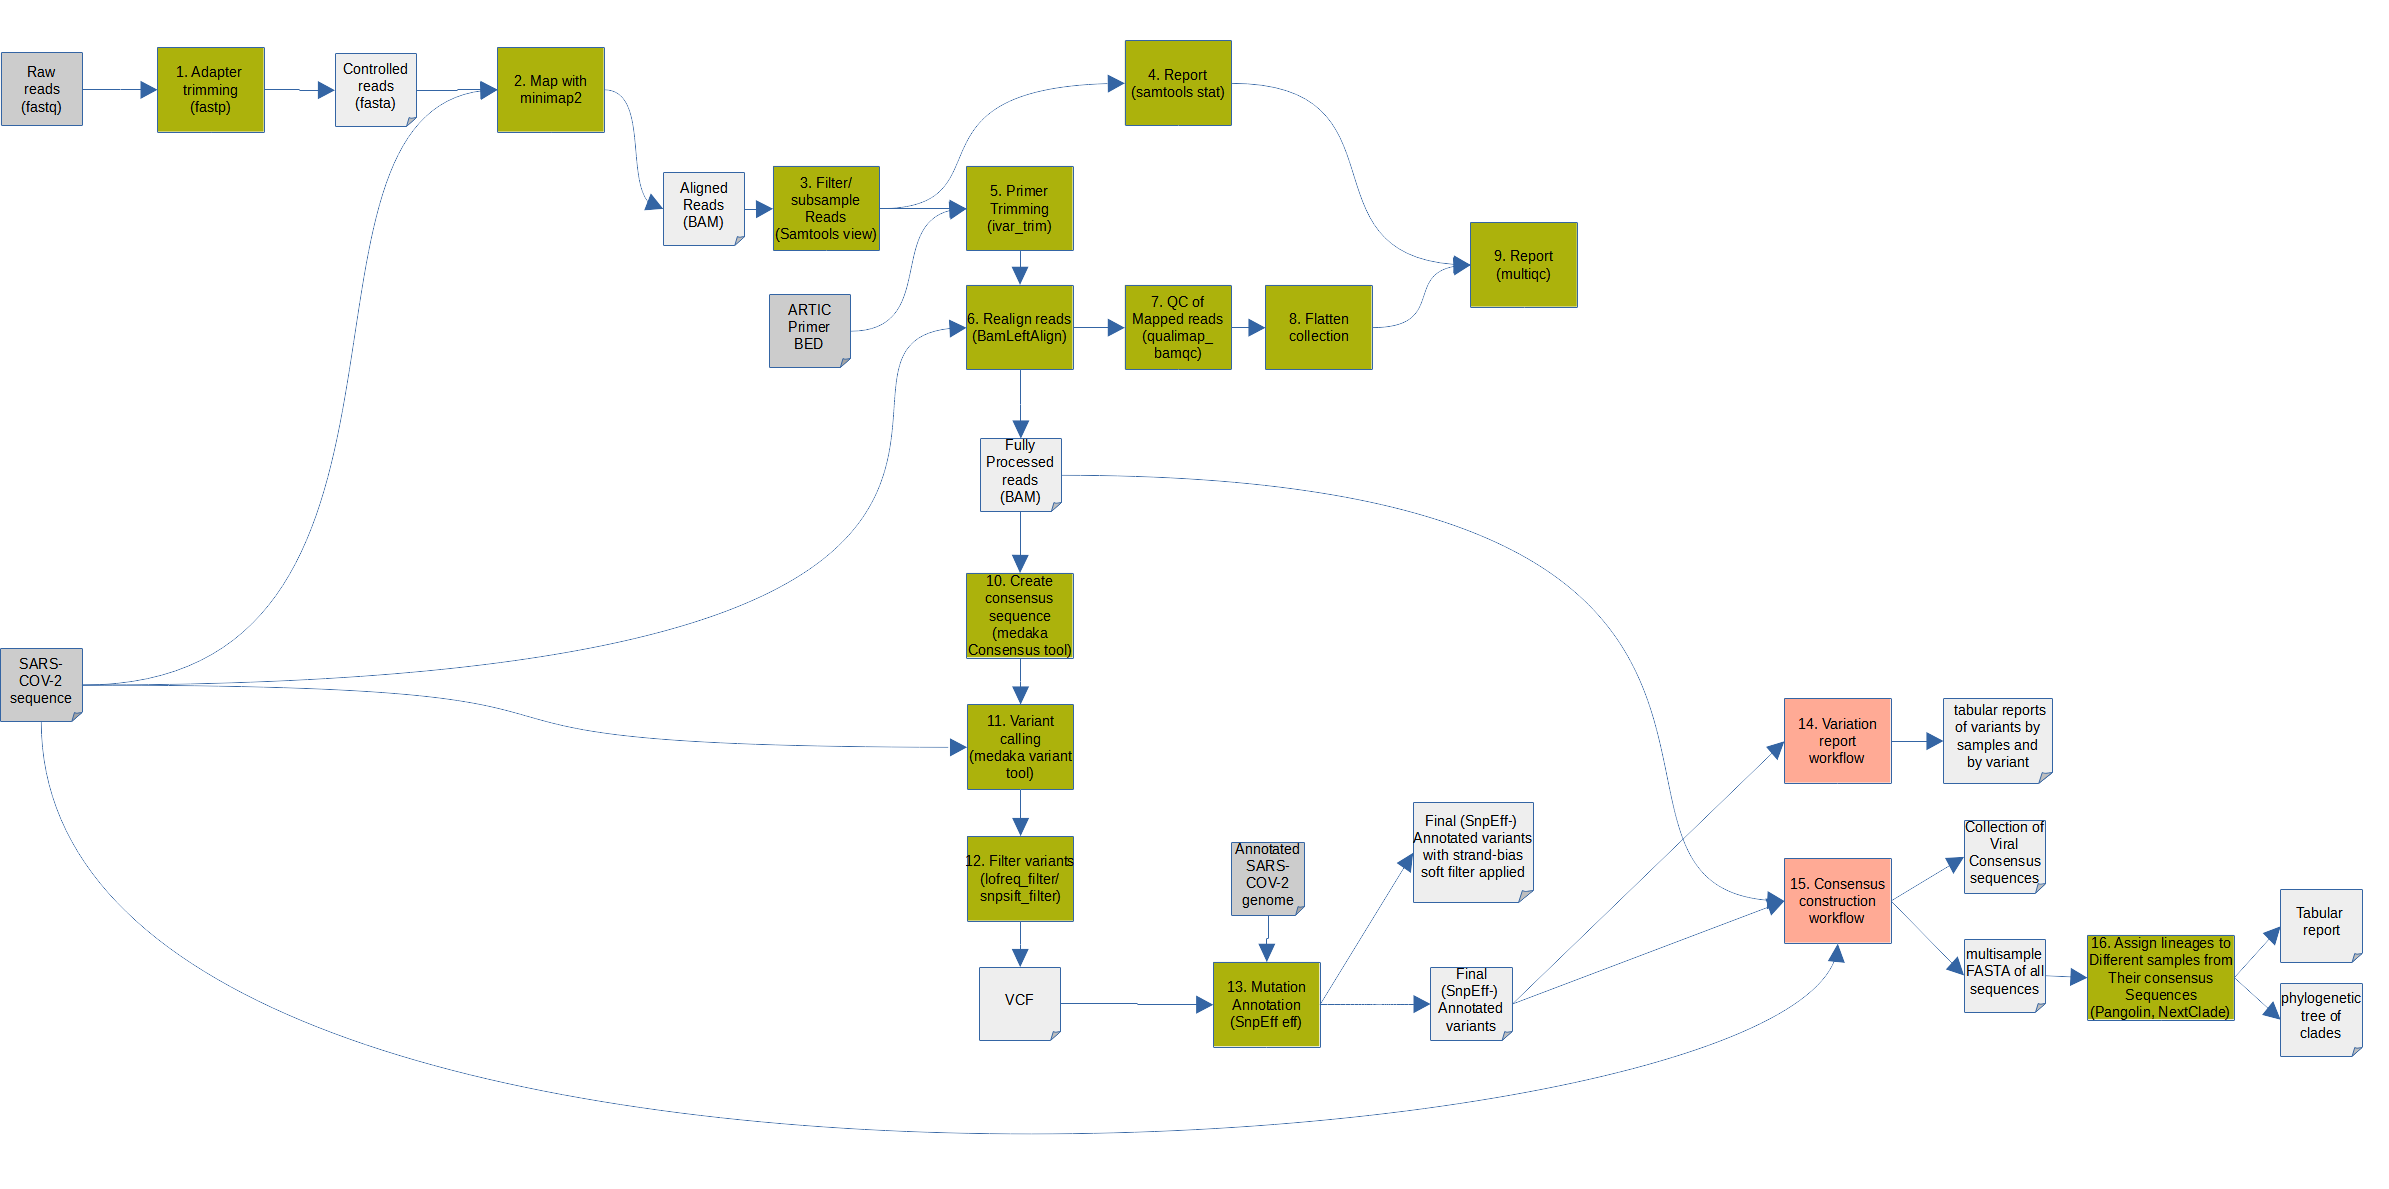
\includegraphics[width=1.4\textwidth]{figures/further/further-ont-wf.png}
            \captionof{figure}{One of four existing Galaxy workflow for SARS-CoV-2 clinical data surveillance for single-end reads data extracted with amplicon-based technique and sequenced with Nanopore sequencing approach.}
            \label{fig:further:ont-wf}
        \end{figure}
        \begin{figure}[ht!]
        	\centering
            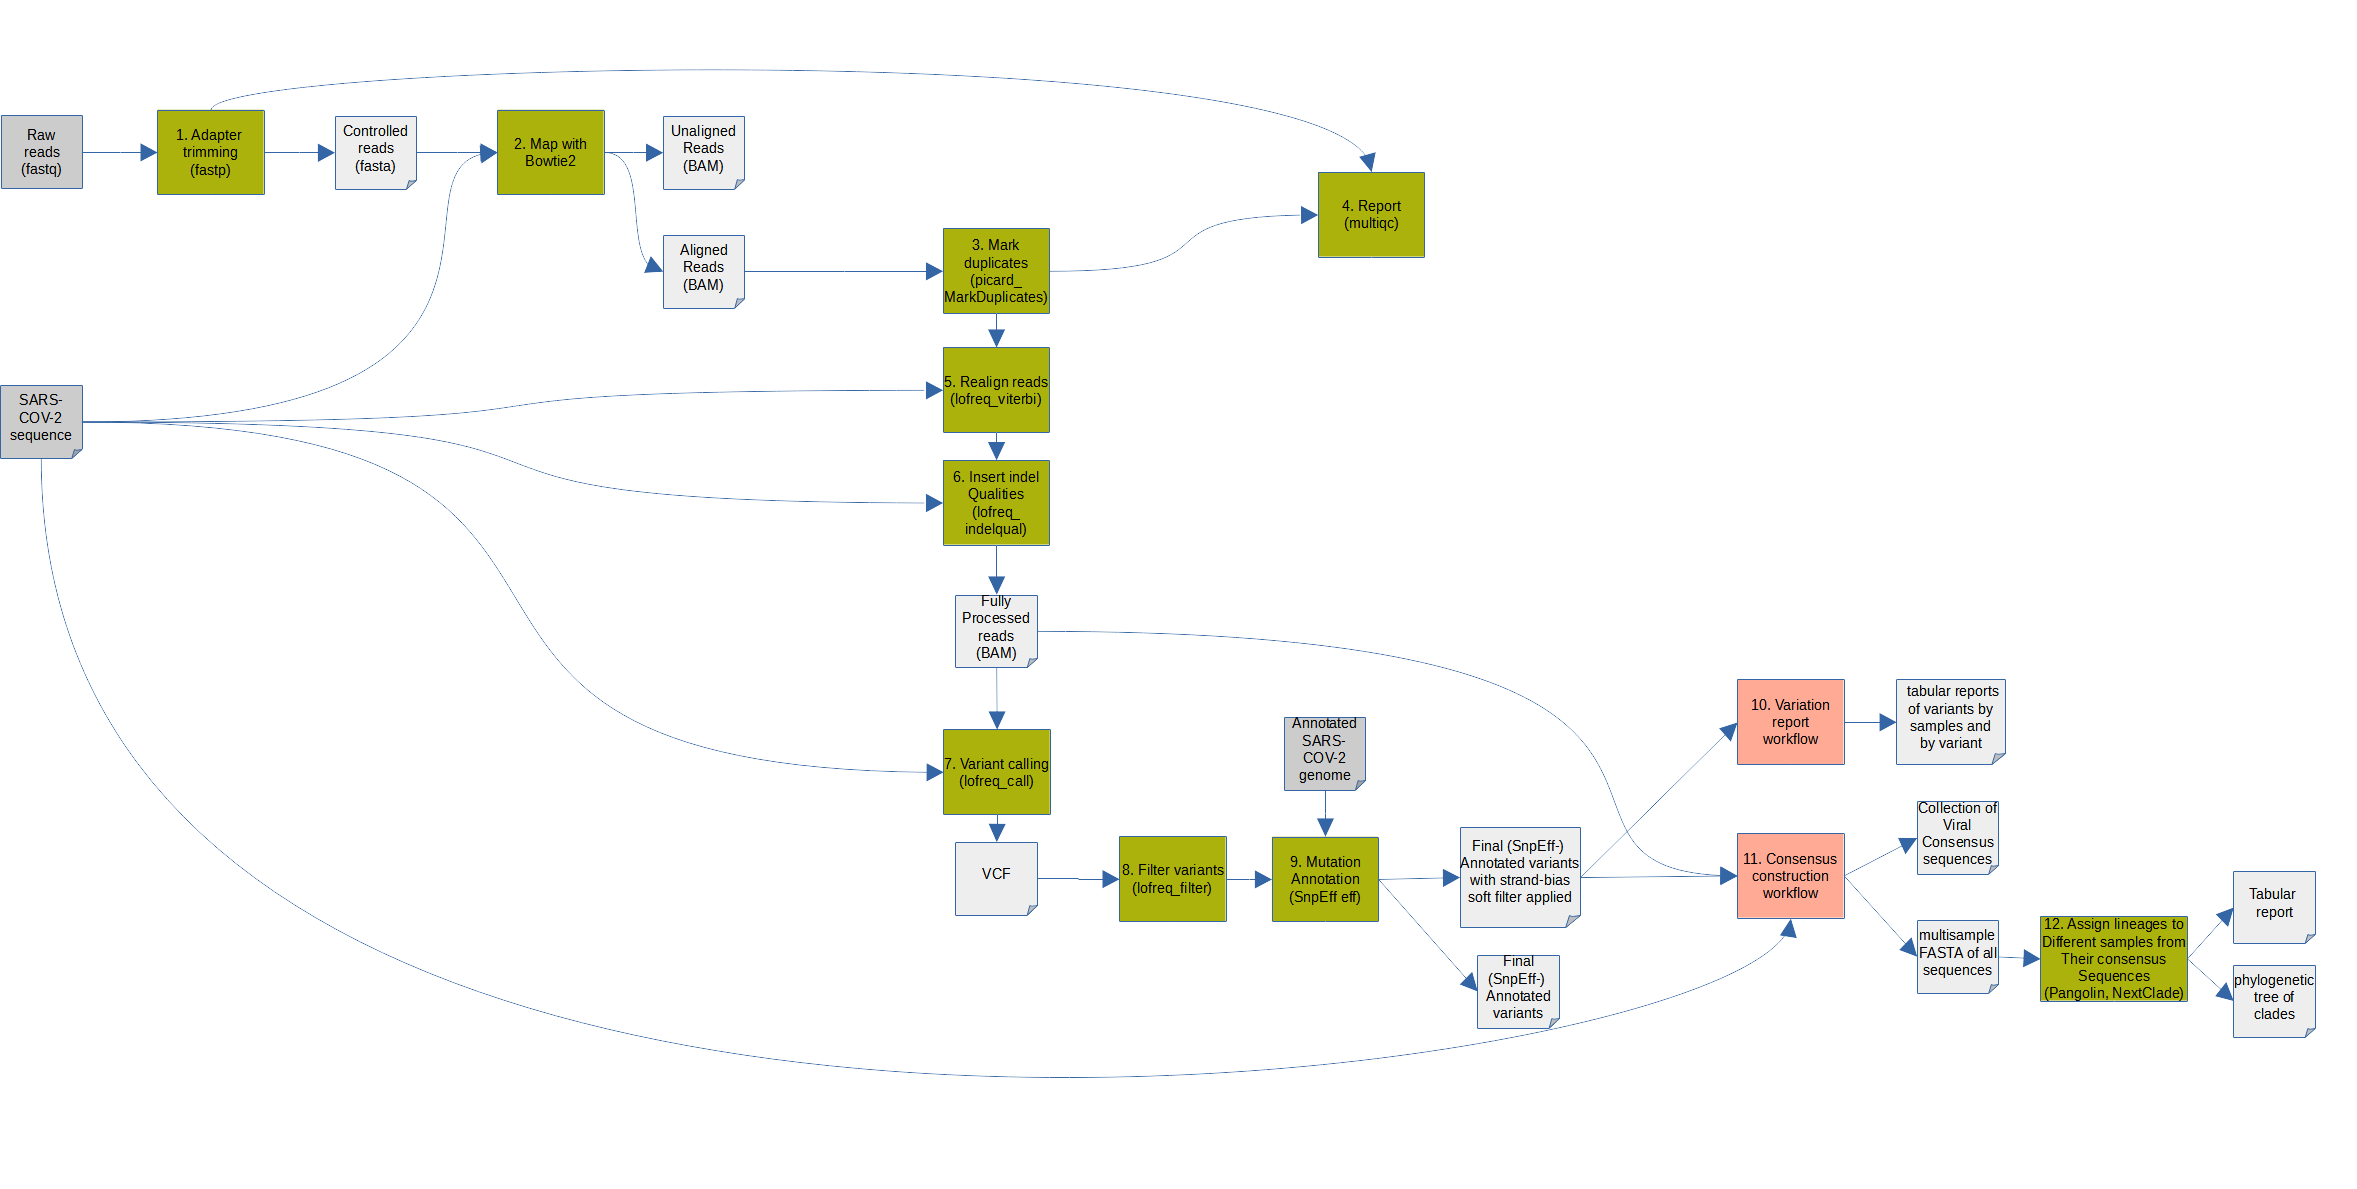
\includegraphics[width=1.4\textwidth]{figures/further/further-illumina-wf.png}
            \captionof{figure}{One of four existing Galaxy workflow for SARS-CoV-2 clinical data surveillance for single-end reads data extracted with metatranscriptomic-based technique and sequenced with Illumina sequencing approach.}
            \label{fig:further:illumina-wf}
        \end{figure}
        \vfill
        \end{landscape}
        
        \subsubsection{Parallel coordinates} 
        \paragraph{Parallel coordinates for all samples} \label{sec:appendix:figures:parallel-all}
        \Cref{fig:further:parallel-delta-all}, \cref{fig:further:parallel-ba1-all} and \cref{fig:further:parallel-ba2-all} depict parallel coordinates for all samples considering only detection of Delta, BA.1, and BA.2 lineage respectively by Freyja and COJAC.
        \begin{figure}[H]
        	\centering
            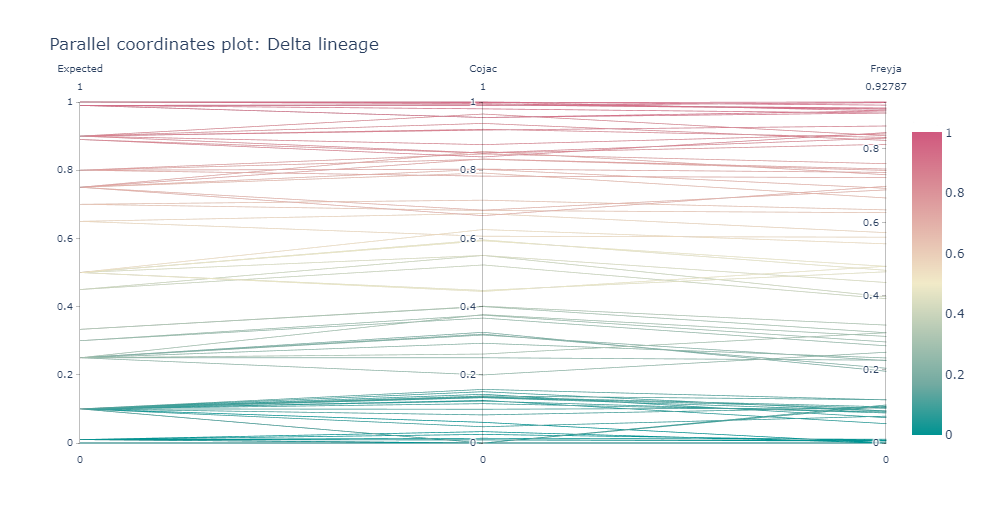
\includegraphics[width=0.8\textwidth]{figures/further/pc-delta-all.png}
            \captionof{figure}{Parallel coordinates plot for all samples that compare Delta lineage proportions detected by Freyja and COJAC with each other as well as with expected proportion. Left axis represents expected proportion of Delta, middle axis represents proportion of Delta lineage detected by COJAC, while right axis represents proportion of Delta lineage detected by Freyja}
            \label{fig:further:parallel-delta-all}
        \end{figure}
        \begin{figure}[H]
        	\centering
            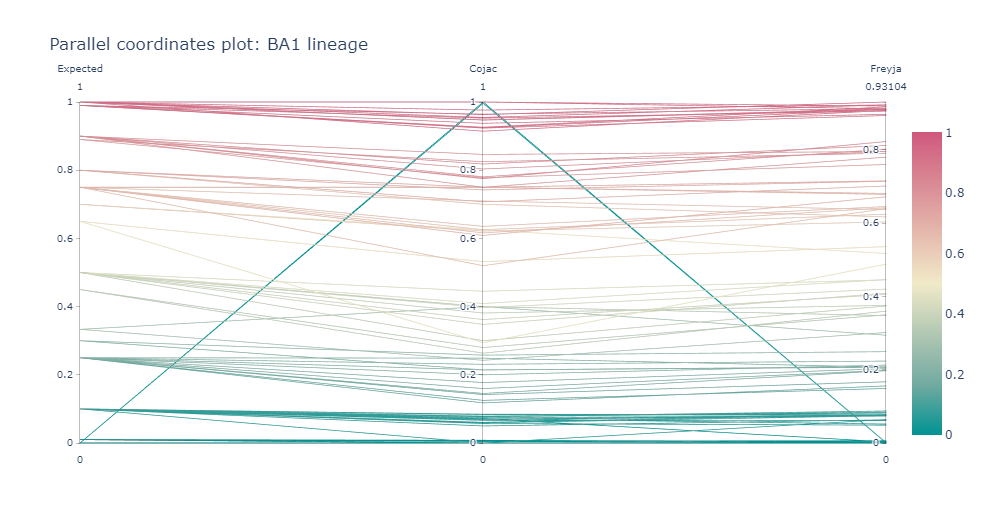
\includegraphics[width=0.8\textwidth]{figures/further/pc-ba1-all.png}
            \captionof{figure}{Parallel coordinates plot for all samples that compare BA.1 lineage proportions detected by Freyja and COJAC with each other as well as with expected proportion. Left axis represents expected proportion of BA.1, middle axis represents proportion of BA.1 lineage detected by COJAC, while right axis represents proportion of BA.1 lineage detected by Freyja}
            \label{fig:further:parallel-ba1-all}
        \end{figure}
        \begin{figure}[H]
        	\centering
            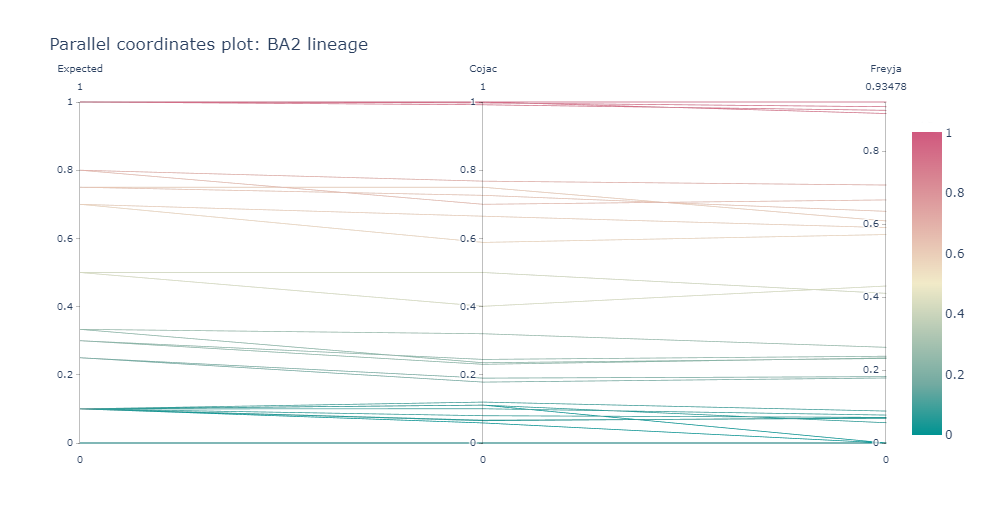
\includegraphics[width=0.8\textwidth]{figures/further/pc-ba2-all.png}
            \captionof{figure}{Parallel coordinates plot for all samples that compare BA.2 lineage proportions detected by Freyja and COJAC with each other as well as with expected proportion. Left axis represents expected proportion of BA.2, middle axis represents proportion of BA.2 lineage detected by COJAC, while right axis represents proportion of BA.2 lineage detected by Freyja}
            \label{fig:further:parallel-ba2-all}
        \end{figure}
        
        \paragraph{Parallel coordinates for samples with two lineages expected} \label{sec:appendix:figures:parallel-twolin}
        \Cref{fig:further:parallel-delta-twolin}, \cref{fig:further:parallel-ba1-twolin} and \cref{fig:further:parallel-ba2-twolin} depict parallel coordinates for "two lineages" group of samples considering only detection of Delta, BA.1, and BA.2 lineage respectively by Freyja and COJAC. Although, for the "two lineages" group of samples, it is not that reasonable to separate graphs into different lineages but focus on the ratio between two expected lineages. Even though, detected proportion of certain expected lineage was worthwhile to to have a look at. Thus, parallel coordinates graphs were generated in the way of one graph per lineage.
        \begin{figure}[H]
        	\centering
            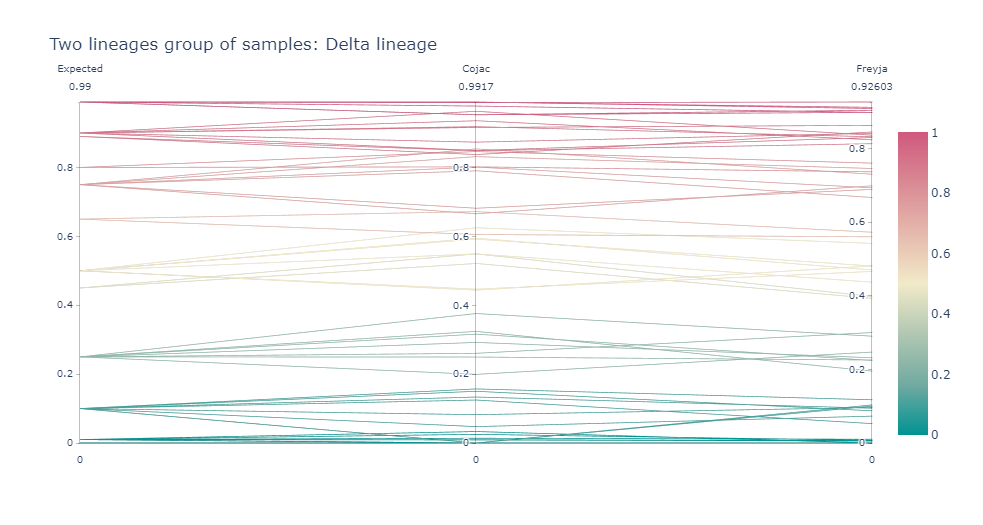
\includegraphics[width=0.8\textwidth]{figures/further/pc-twolin-delta.png}
            \captionof{figure}{Parallel coordinates plot for "two lineages group" of samples that compare Delta lineage proportions detected by Freyja and COJAC with each other as well as with expected proportion. Left axis represents expected proportion of Delta, middle axis represents proportion of Delta lineage detected by COJAC, while right axis represents proportion of Delta lineage detected by Freyja}
            \label{fig:further:parallel-delta-twolin}
        \end{figure}
        \begin{figure}[H]
        	\centering
            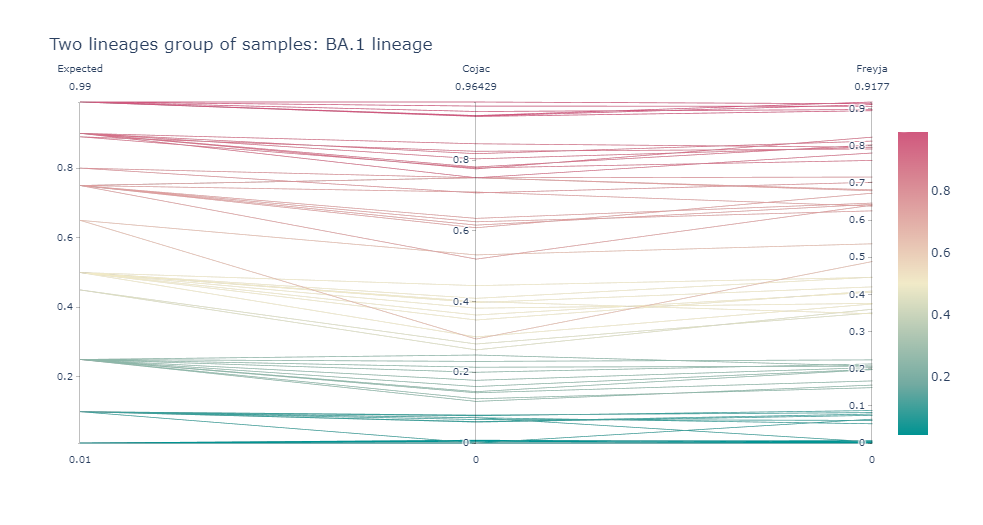
\includegraphics[width=0.8\textwidth]{figures/further/pc-twolin-ba1.png}
            \captionof{figure}{Parallel coordinates plot for "two lineages group" of samples that compare BA.1 lineage proportions detected by Freyja and COJAC with each other as well as with expected proportionfor "two lineages group" of samples. Left axis represents expected proportion of BA.1, middle axis represents proportion of BA.1 lineage detected by COJAC, while right axis represents proportion of BA.1 lineage detected by Freyja}
            \label{fig:further:parallel-ba1-twolin}
        \end{figure}
        \begin{figure}[H]
        	\centering
            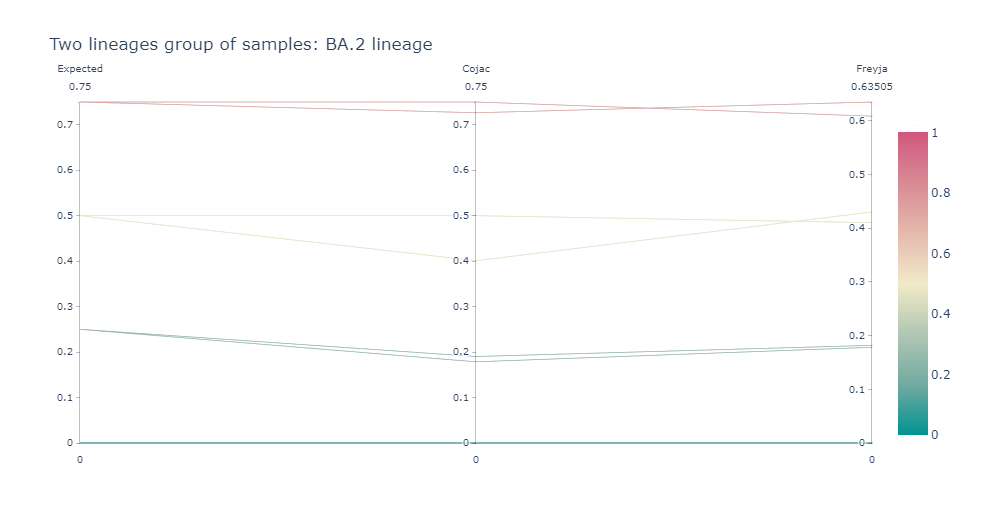
\includegraphics[width=0.8\textwidth]{figures/further/pc-twolin-ba2.png}
            \captionof{figure}{Parallel coordinates plot for "two lineages group" of samples that compare BA.2 lineage proportions detected by Freyja and COJAC with each other as well as with expected proportion for "two lineages group" of samples. Left axis represents expected proportion of BA.2, middle axis represents proportion of BA.2 lineage detected by COJAC, while right axis represents proportion of BA.2 lineage detected by Freyja}
            \label{fig:further:parallel-ba2-twolin}
        \end{figure}
        
        \subsubsection{Example of different types of plots for one sample} 
        \Cref{fig:further:bar-s1}, \cref{fig:further:pc-s1} and \cref{fig:further:line-s1} show plots generated per sample to make detailed observations. The example for the sample1 is provided below. However, these graphs were constructed for every sample during this master thesis. Types of plots that were generated per one sample: i) bar plot (\cref{fig:further:bar-s1}); ii) parallel coordinates plot (\cref{fig:further:pc-s1}); iii) line plot (\cref{fig:further:line-s1}), to look at absolute values of lineage proportion against scaled values in parallel coordinates. The comparison with expected lineage proportions was included in these plots.
.
        \begin{figure}[H]
        	\centering
            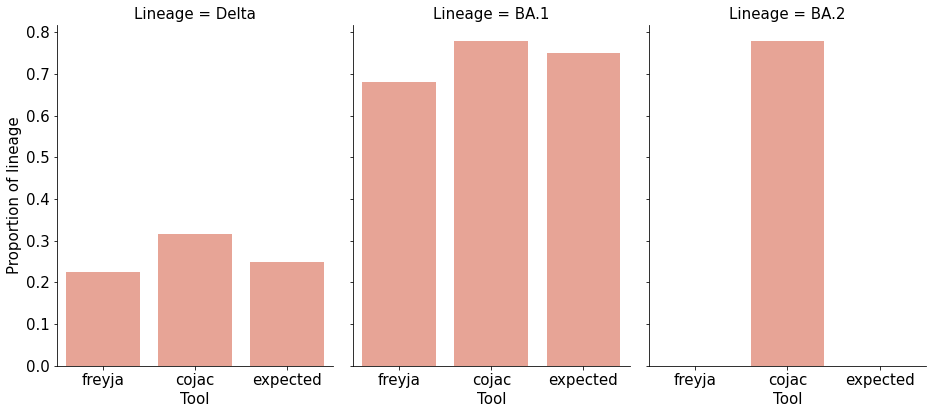
\includegraphics[width=0.8\textwidth]{figures/further/bar-s1.png}
            \captionof{figure}{Bar plot for sample 1.}
            \label{fig:further:bar-s1}
        \end{figure}
        \begin{figure}[H]
        	\centering
            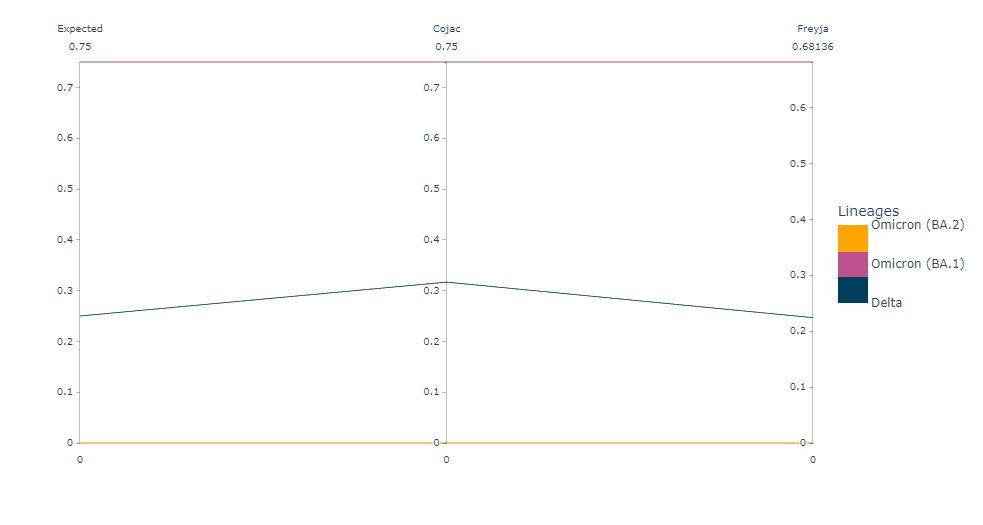
\includegraphics[width=0.8\textwidth]{figures/further/pc-s1.png}
            \captionof{figure}{Parallel coordinates plot for sample 1}
            \label{fig:further:pc-s1}
        \end{figure}
        \begin{figure}[H]
        	\centering
            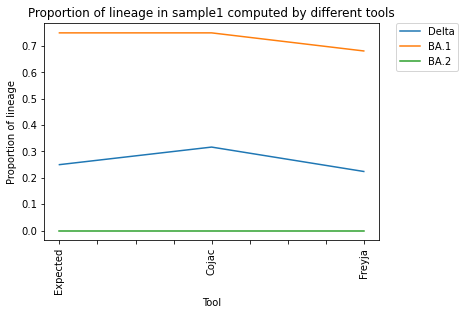
\includegraphics[width=0.8\textwidth]{figures/further/line-s1.png}
            \captionof{figure}{Line plot for sample 1}
            \label{fig:further:line-s1}
        \end{figure}
        
        \subsubsection{Collection of bar plots across all samples is provided} \label{sec:appendix:figures:bars-all}
        \Cref{fig:further:bars-delta-all}, \cref{fig:further:bars-ba1-all} and \cref{fig:further:bars-ba2-all} depict barplots for all samples considering only detection of Delta, BA.1, and BA.2 lineage respectively.
        
        \begin{figure}[H]
        	\centering
            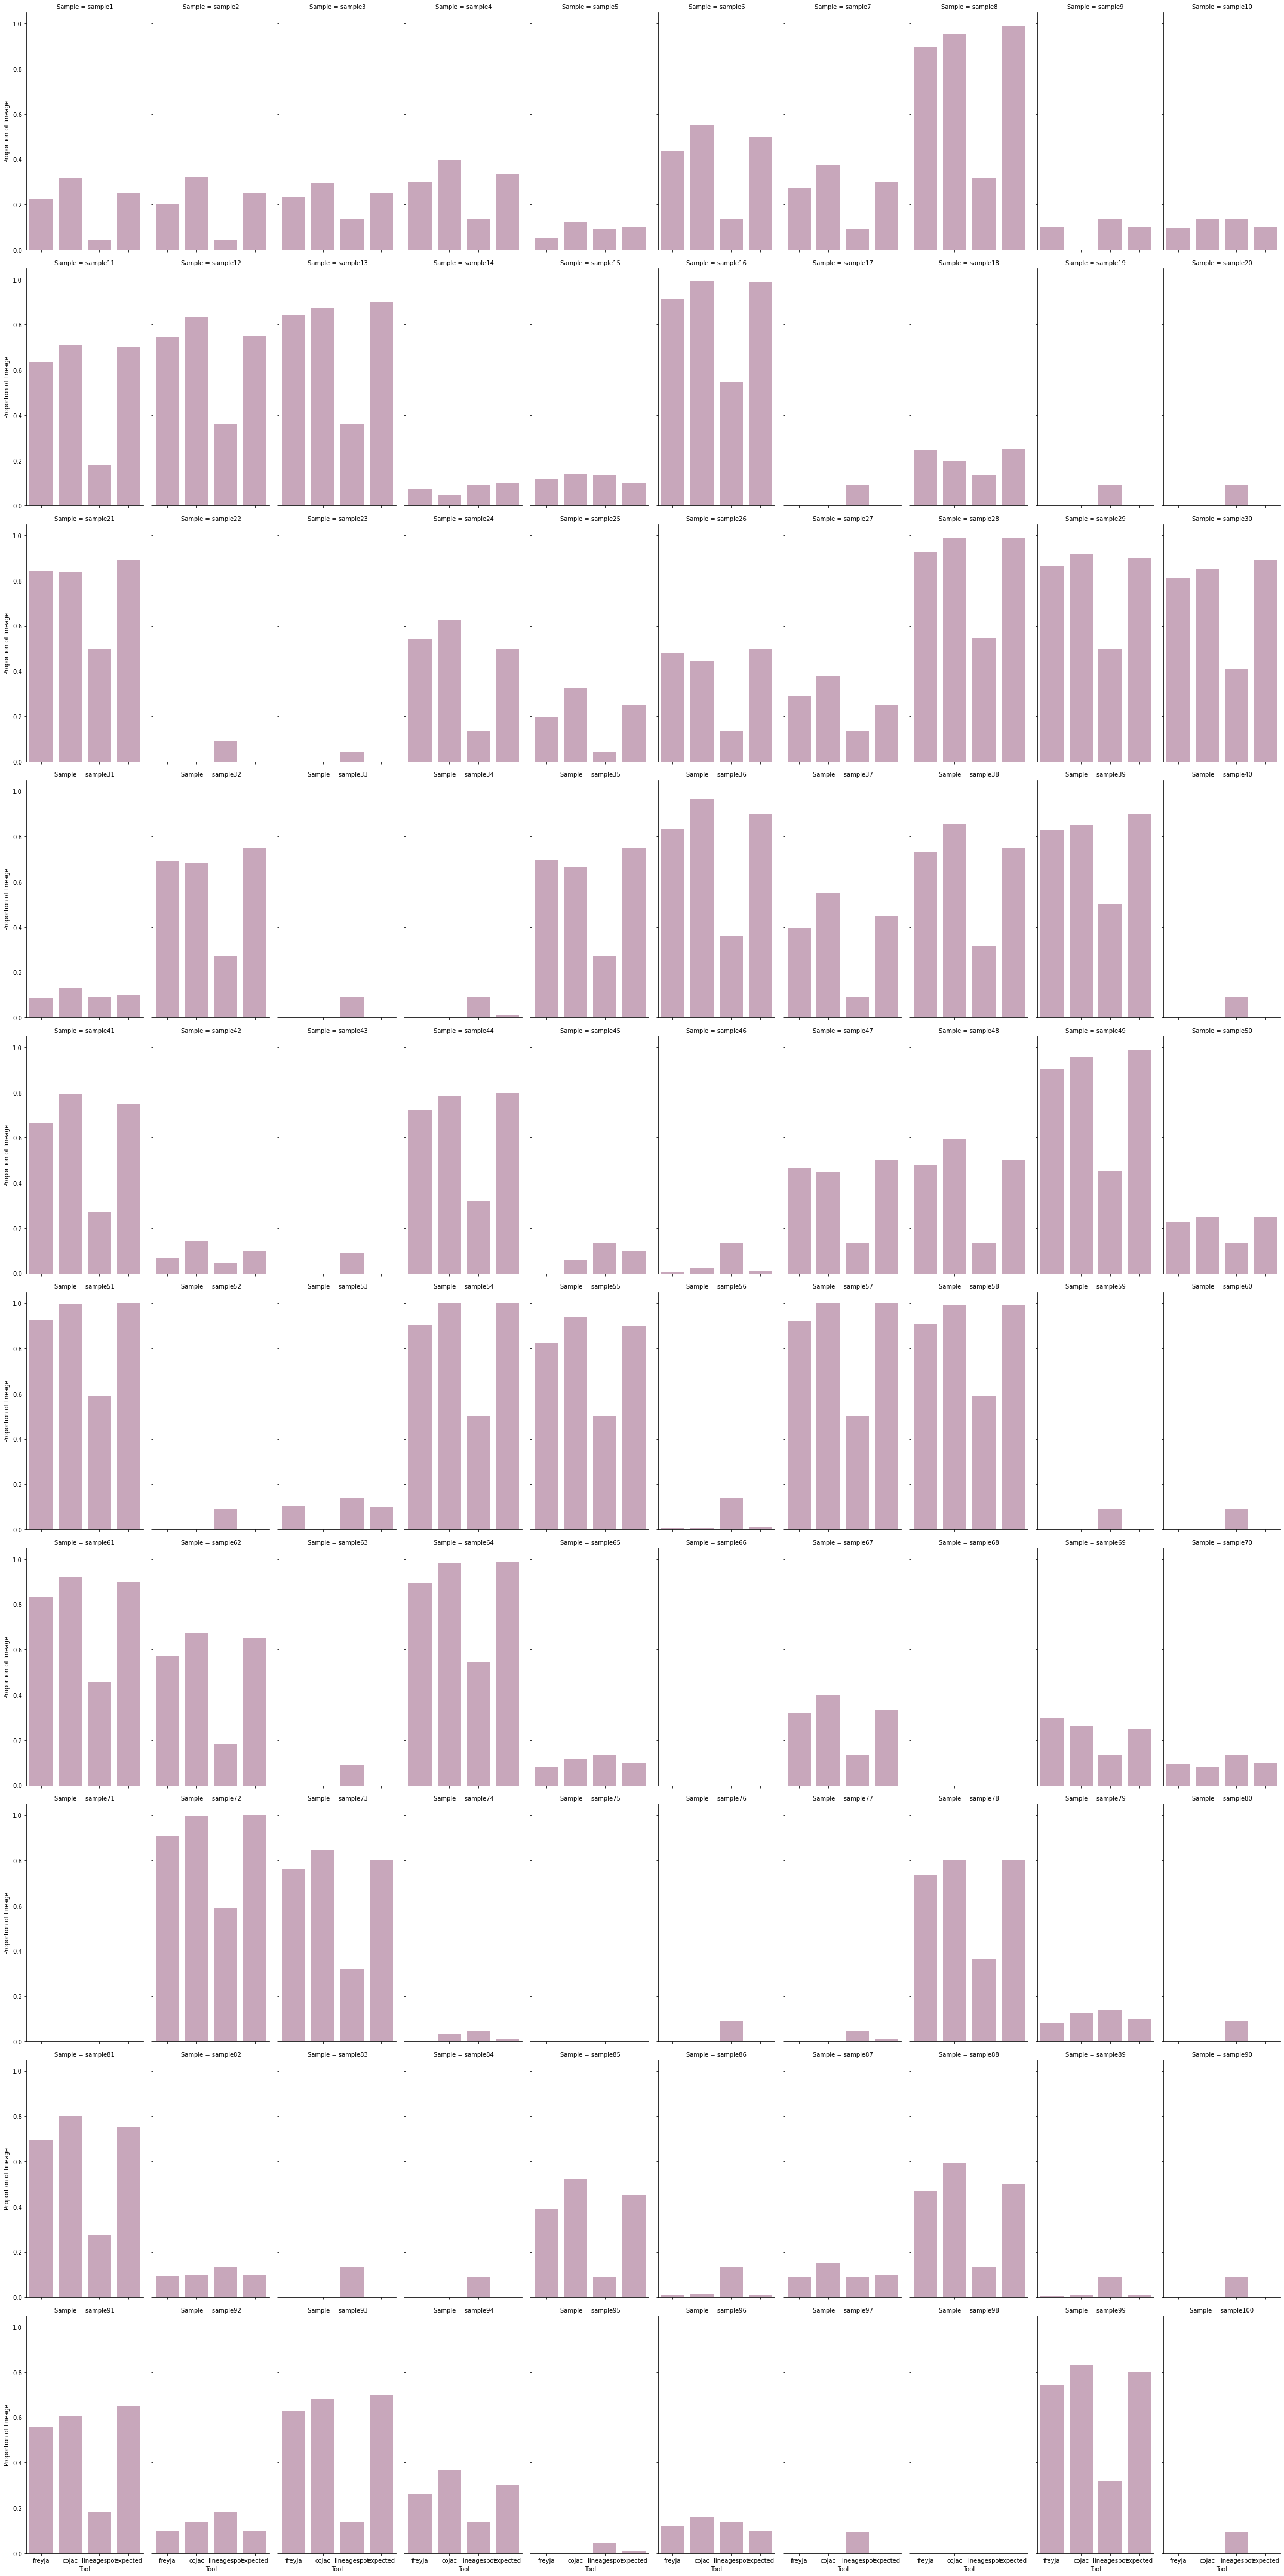
\includegraphics[width=0.7\textwidth]{figures/further/bars-delta-all.png}
            \captionof{figure}{Bar plots that compare Delta lineage proportions detected by Freyja and COJAC with each other as well as with expected proportion.}
            \label{fig:further:bars-delta-all}
        \end{figure}
        \begin{figure}[H]
        	\centering
            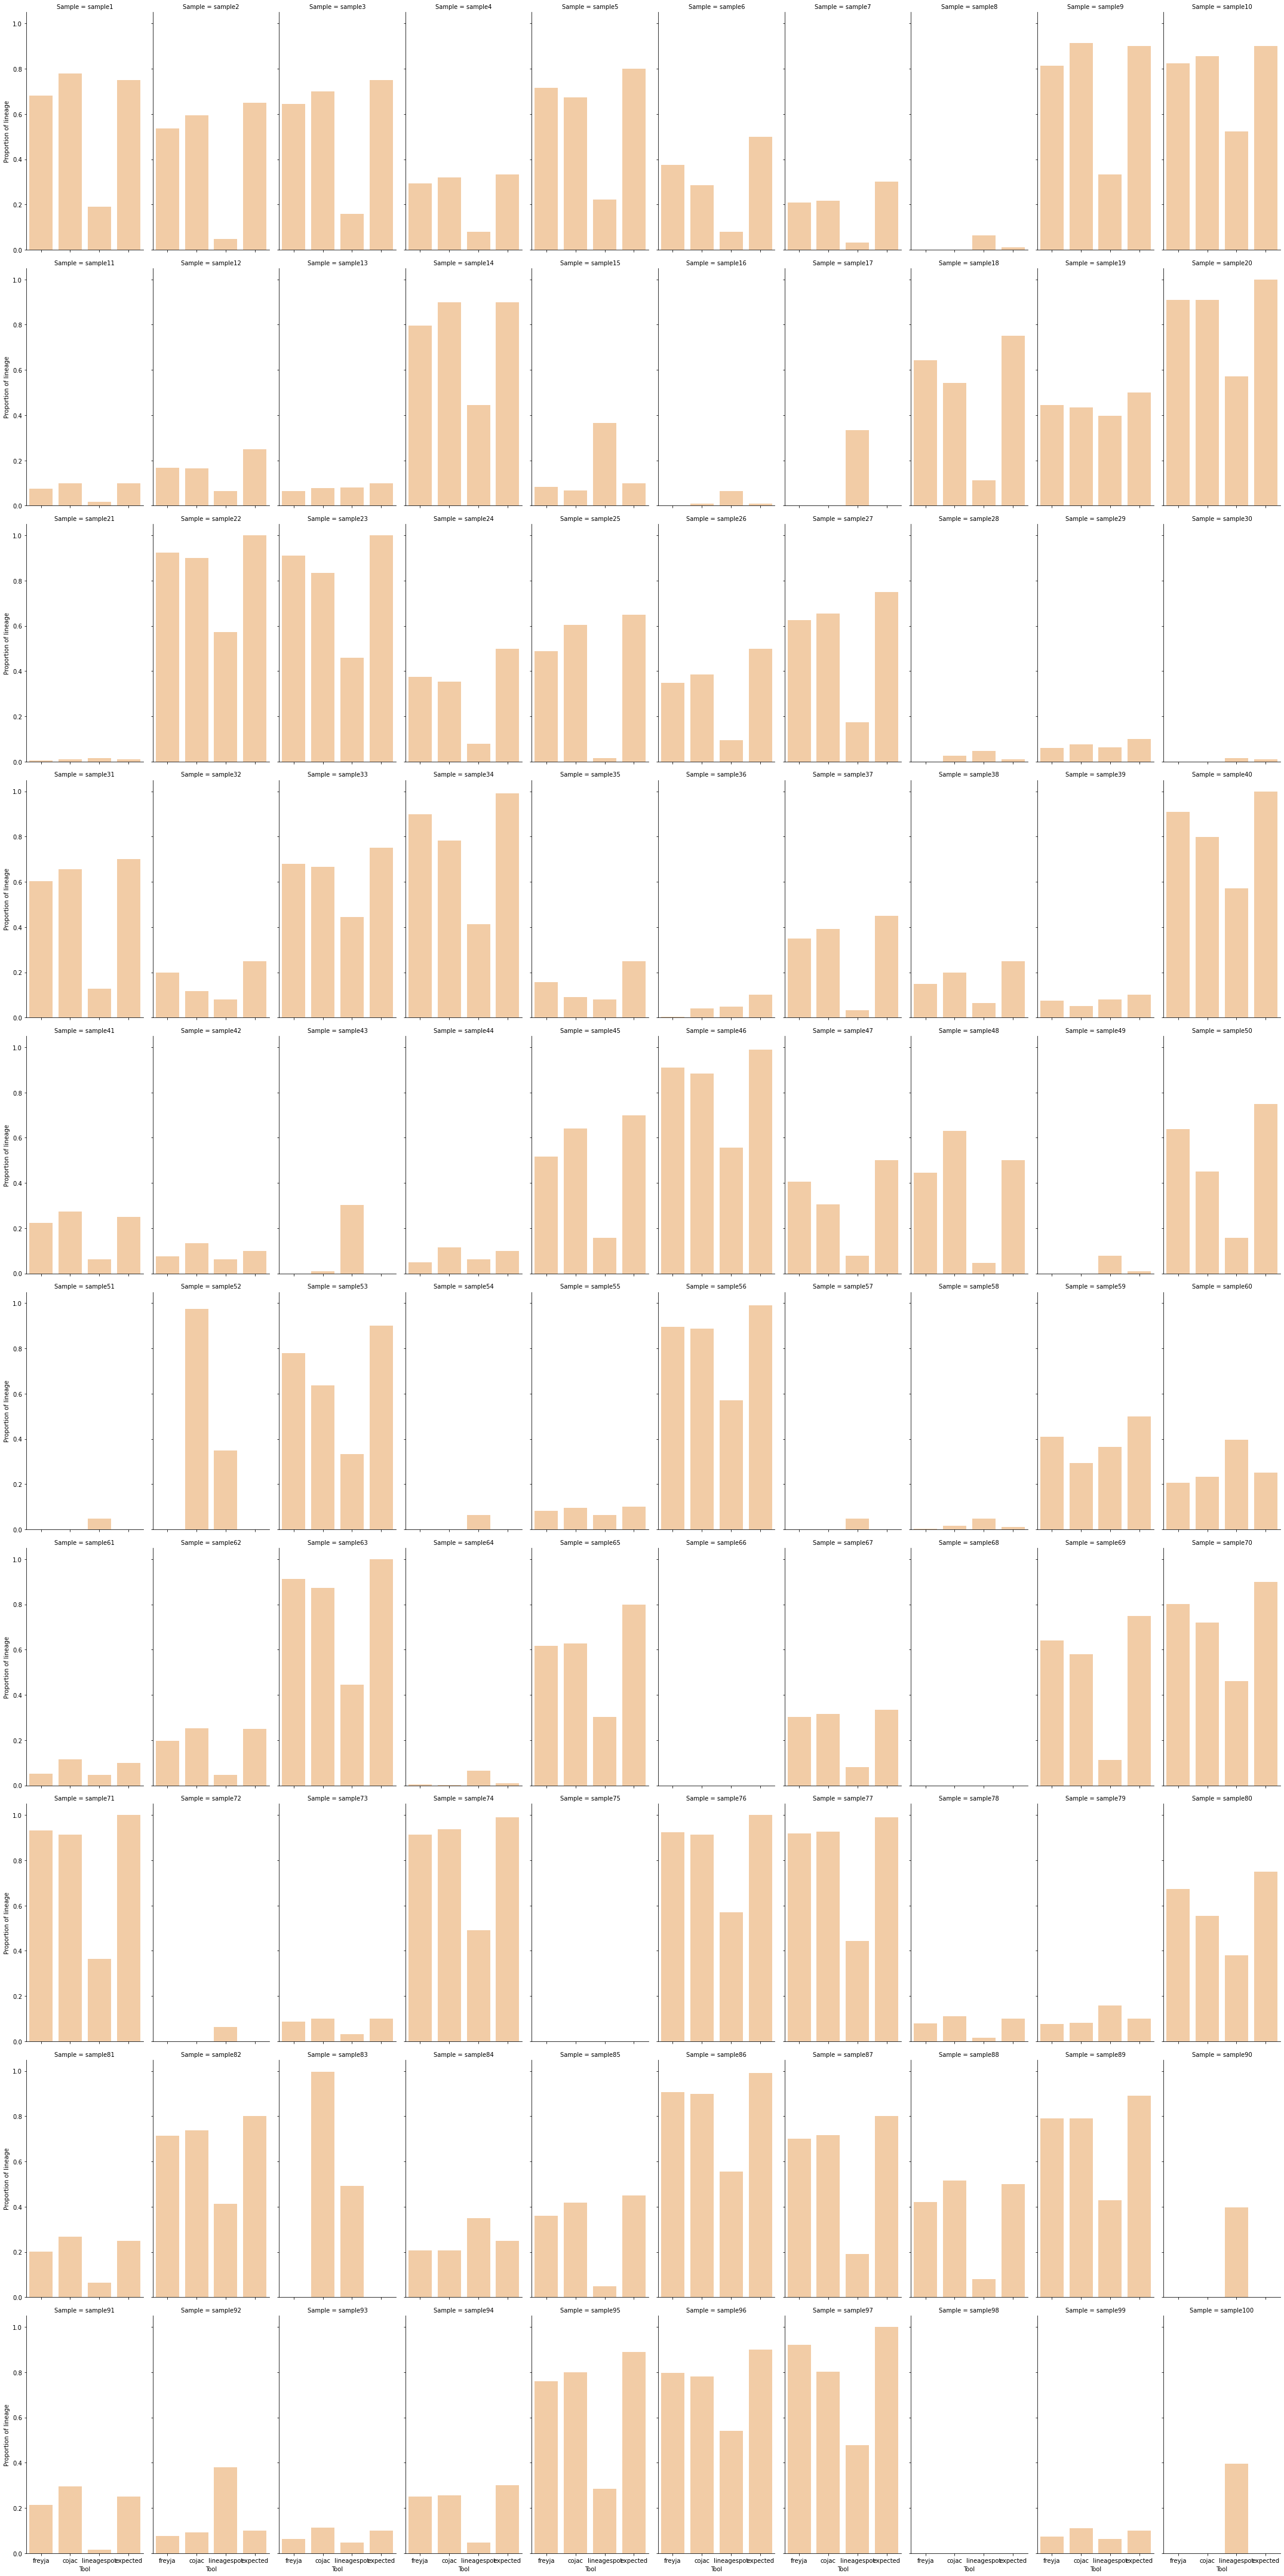
\includegraphics[width=0.7\textwidth]{figures/further/bars-ba1-all.png}
            \captionof{figure}{Bar plots that compare BA.1 lineage proportions detected by Freyja and COJAC with each other as well as with expected proportion}
            \label{fig:further:bars-ba1-all}
        \end{figure}
        \begin{figure}[H]
        	\centering
            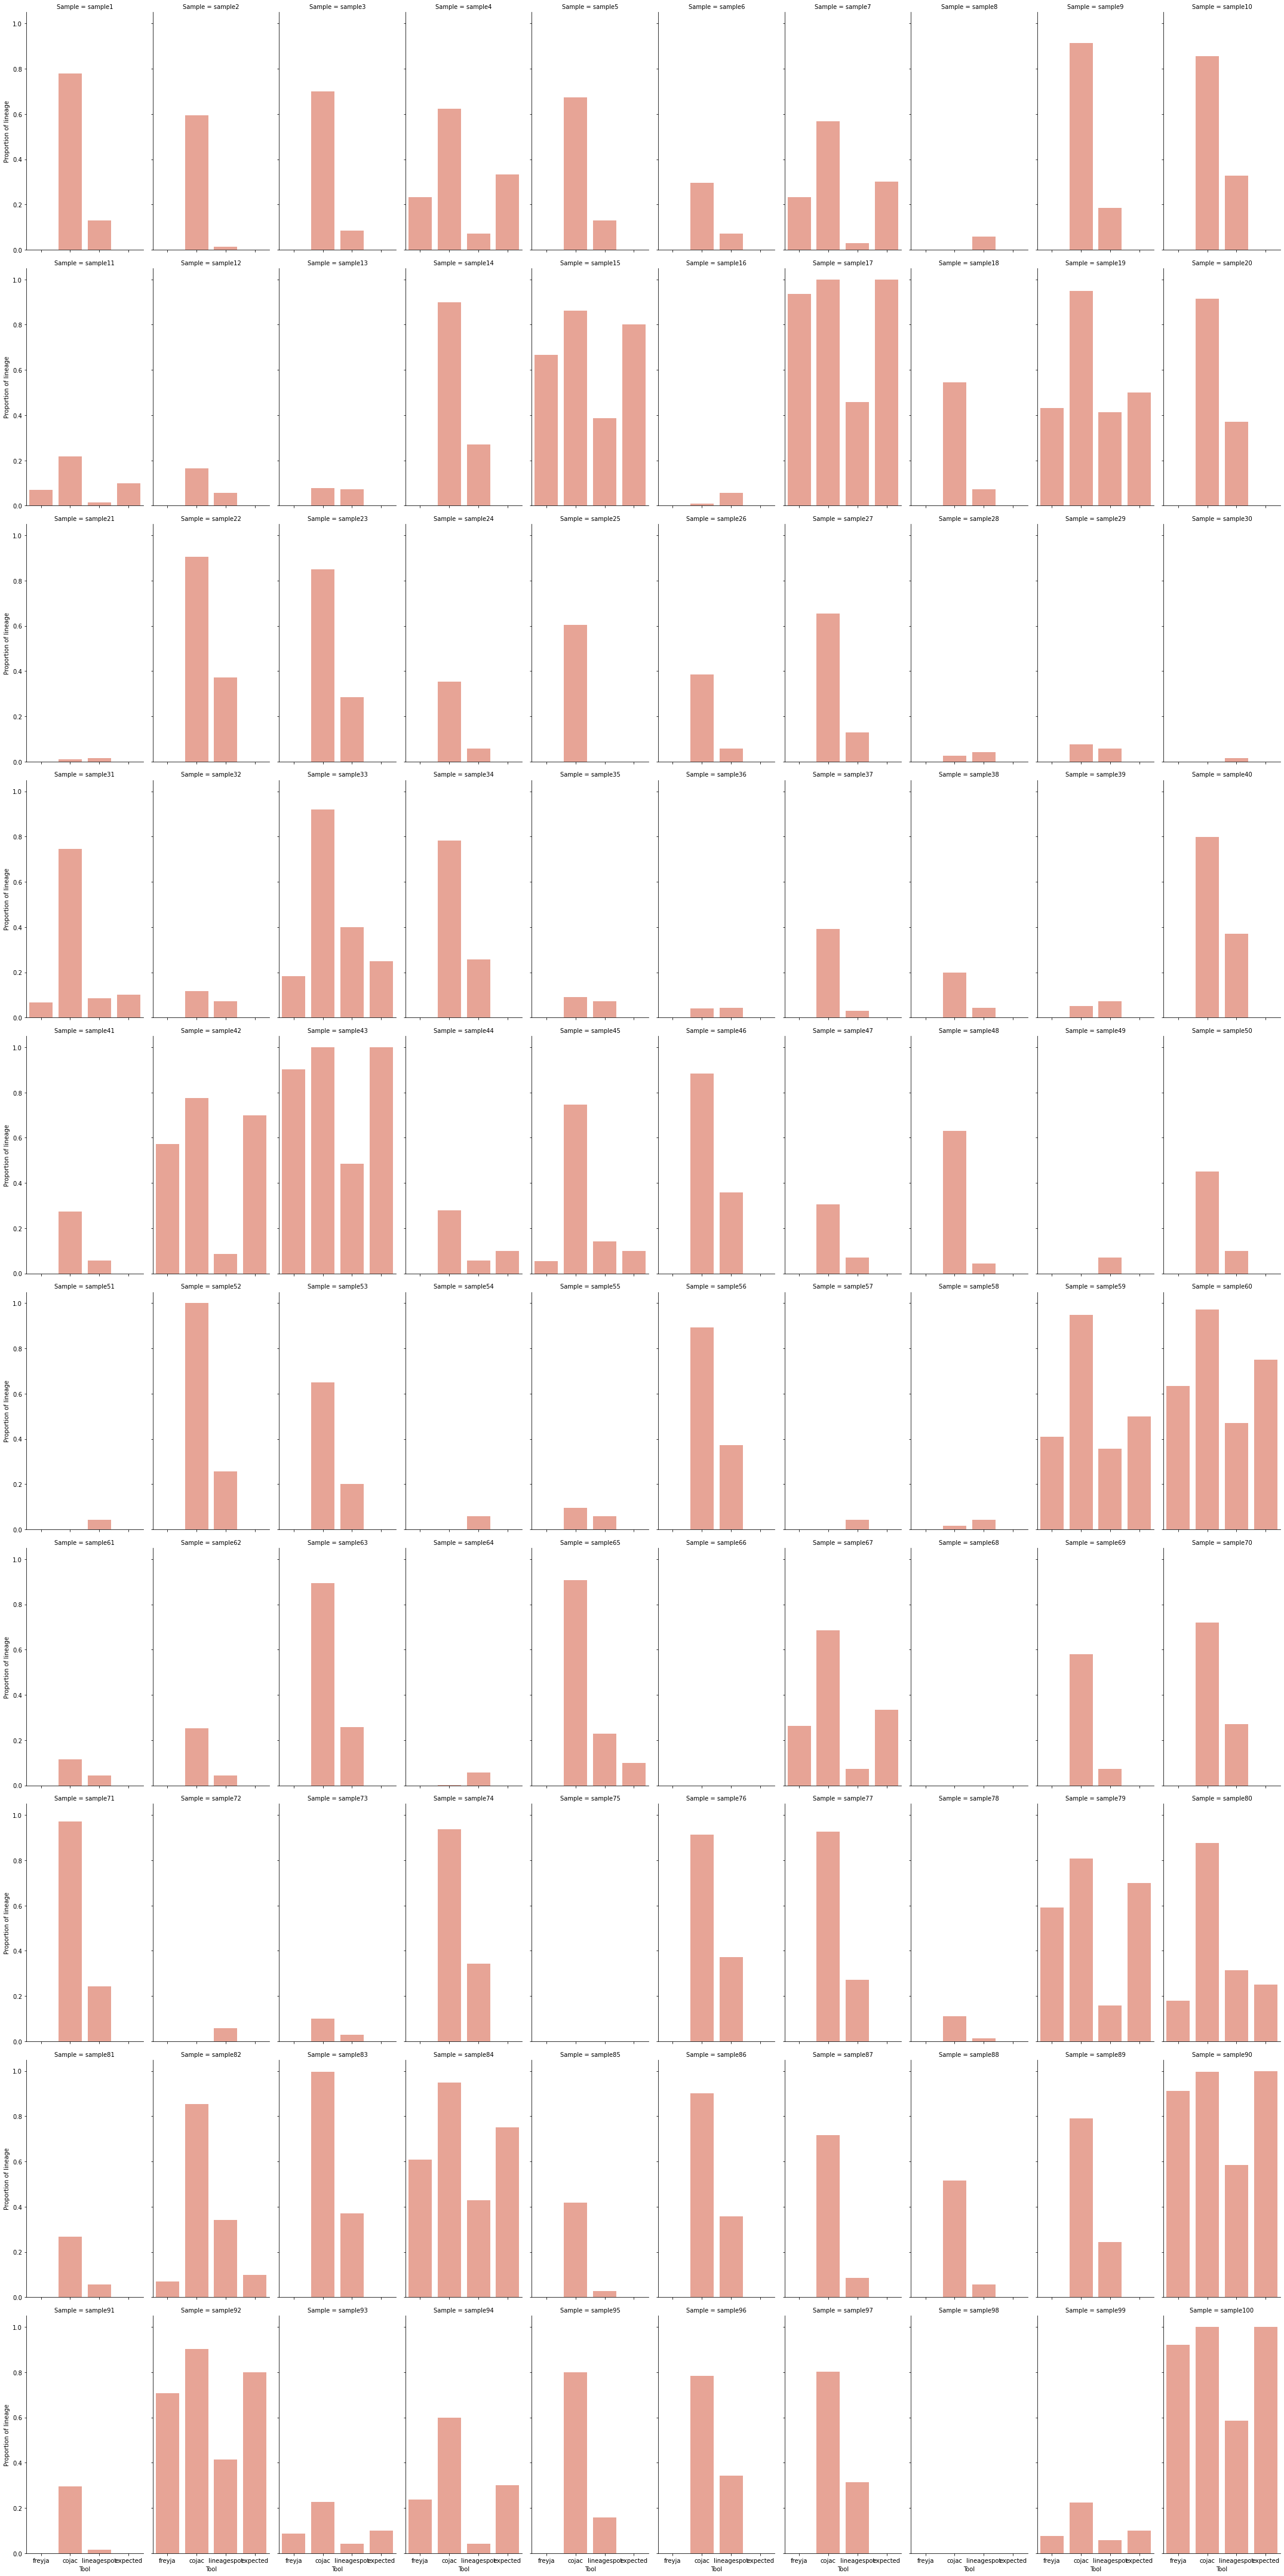
\includegraphics[width=0.7\textwidth]{figures/further/bars-ba2-all.png}
            \captionof{figure}{Bar plots that compare BA.2 lineage proportions detected by Freyja and COJAC with each other as well as with expected proportion.}
            \label{fig:further:bars-ba2-all}
        \end{figure}
        
       \subsubsection{Distribution of lineages proportions detected by Lineagespot across all mock samples}  
        \Cref{fig:further:dist-ls} represents the proportions of every lineage detected by Lineagespot on mock dataset. Observed that most of the samples, more than 50\%, according to Lineagespot, carry a small proportion, no more than 0.15, of lineage abundance, while higher proportions of all 3 lineages are present in less amount of samples. 
        
        Fig.10. all three considered lineages (Delta, BA.1, BA.2) proportion distribution among results detected by Lineagespot.
        \begin{figure}[H]
        	\centering
            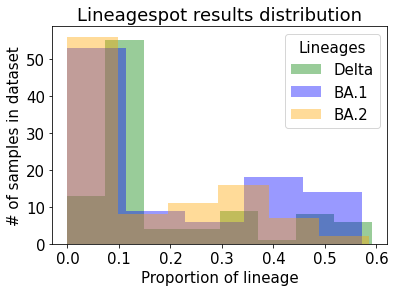
\includegraphics[width=0.5\textwidth]{figures/further/distr-lineagespot.png}
            \captionof{figure}{All three considered lineages (Delta, BA.1, BA.2) proportion distribution among results detected by Lineagespot on mock dataset.}
            \label{fig:further:dist-ls}
        \end{figure}
        
\clearpage

